\documentclass[12pt,a4paper]{article}

% =================== PACKAGES ===================
\usepackage[utf8]{inputenc}
\usepackage[T1]{fontenc}
\usepackage[french]{babel}
\usepackage{amsmath,amssymb,amsfonts}
\usepackage{graphicx}
\usepackage{hyperref}
\usepackage{booktabs}
\usepackage{array}
\usepackage{multirow}
\usepackage{colortbl}
\usepackage{xcolor}
\usepackage{fancyhdr}
\usepackage{geometry}
\usepackage{titlesec}
\usepackage{caption}
\usepackage{subcaption}
\usepackage{listings}
\usepackage{float}
\usepackage{tabularx}
\usepackage{enumitem}
\usepackage{tikz}
\usepackage{pgfplots}
\pgfplotsset{compat=1.18}

% =================== MISE EN PAGE ===================
\geometry{top=2.5cm, bottom=2.5cm, left=2.5cm, right=2.5cm}
\setlength{\parskip}{6pt}
\setlength{\parindent}{0pt}

% =================== STYLE DES SECTIONS ===================
\titleformat{\section}{\Large\bfseries\color{blue!60!black}}{}{0em}{}
\titleformat{\subsection}{\large\bfseries\color{blue!50!black}}{}{0em}{}
\titleformat{\subsubsection}{\normalsize\bfseries\color{blue!40!black}}{}{0em}{}

% =================== EN-TETE ET PIED DE PAGE ===================
\pagestyle{fancy}
\fancyhf{}
\fancyhead[L]{\small Détection d'Intrusion Réseau}
\fancyhead[R]{\small Projet ML - Cybersécurité}
\fancyfoot[C]{\thepage}
\renewcommand{\headrulewidth}{0.4pt}

% =================== CODE COULEURS ===================
\definecolor{codegreen}{rgb}{0,0.6,0}
\definecolor{codegray}{rgb}{0.5,0.5,0.5}
\definecolor{codepurple}{rgb}{0.58,0,0.82}
\definecolor{backcolour}{rgb}{0.95,0.95,0.92}

\lstdefinestyle{mystyle}{
    backgroundcolor=\color{backcolour},
    commentstyle=\color{codegreen},
    keywordstyle=\color{magenta},
    numberstyle=\tiny\color{codegray},
    stringstyle=\color{codepurple},
    basicstyle=\ttfamily\footnotesize,
    breakatwhitespace=false,
    breaklines=true,
    captionpos=b,
    keepspaces=true,
    numbers=left,
    numbersep=5pt,
    showspaces=false,
    showstringspaces=false,
    showtabs=false,
    tabsize=2
}
\lstset{style=mystyle}

% =================== DOCUMENT ===================
\begin{document}

% =================== PAGE DE GARDE ===================
\begin{titlepage}
    \centering
    \vspace*{1cm}

    \begin{tikzpicture}
        \shade[top color=blue!60, bottom color=blue!20] (0,0) rectangle (\textwidth,0.3);
    \end{tikzpicture}

    \vspace{0.5cm}

    {\LARGE \textbf{Université Paris-Saclay}\par}
    \vspace{0.3cm}
    {\Large L2 IAD - S4 \par}
    \vspace{0.5cm}

    \begin{tikzpicture}
        \shade[top color=blue!20, bottom color=blue!60] (0,0) rectangle (\textwidth,0.3);
    \end{tikzpicture}

    \vspace{2cm}

    {\Huge \textbf{Détection d'Intrusion Réseau}\par}
    \vspace{0.5cm}
    {\Large par Machine Learning\par}

    \vspace{1.5cm}

    {\LARGE \textbf{Classification d'Attaques}\par}
    {\Large avec le Dataset NSL-KDD\par}

    \vspace{2cm}

    \begin{minipage}{0.8\textwidth}
        \centering
        \large
        \textbf{Projet de Machine Learning et Cybersécurité}\par
        \vspace{0.5cm}
        \textbf{Auteur :} [Votre Nom]\par
        \textbf{Date :} Mai 2026\par
        \textbf{Encadrant :} [Nom du Professeur]\par
    \end{minipage}

    \vspace{2cm}

    \begin{tikzpicture}
        \shade[top color=blue!60, bottom color=blue!20] (0,0) rectangle (\textwidth,0.3);
    \end{tikzpicture}

    \vfill
\end{titlepage}

% =================== TABLE DES MATIERES ===================
\newpage
\tableofcontents
\newpage

% =================== INTRODUCTION ===================
\section{Introduction}

\subsection{Contexte et Problématique}

Dans le contexte actuel de transformation numérique, les entreprises sont confrontées à une augmentation constante des menaces informatiques. Les attaques réseau représentent l'une des principales préoccupations des équipes de cybersécurité. La détection rapide et précise de ces intrusions est devenue un enjeu critique pour la protection des infrastructures et des données sensibles.

Les systèmes de détection d'intrusion (IDS - Intrusion Detection System) traditionnels reposent sur des règles définies manuellement par des experts en sécurité. Bien qu'efficaces contre les attaques connues, ces approches montrent leurs limites face aux attaques émergentes et aux variations des patterns malveillants.

\subsection{Objectifs du Projet}

Ce projet vise à développer un système de détection d'intrusion réseau basé sur des techniques de Machine Learning. Plus spécifiquement, les objectifs sont :

\begin{itemize}
    \item \textbf{Analyser} le dataset NSL-KDD pour comprendre les caractéristiques du trafic réseau normal et malveillant
    \item \textbf{Prétraiter} les données (encodage, normalisation, équilibrage des classes)
    \item \textbf{Entraîner} plusieurs modèles de classification supervisée
    \item \textbf{Évaluer} et comparer les performances des différents modèles
    \item \textbf{Déployer} une interface de prédiction temps réel avec Streamlit
\end{itemize}

\subsection{Organisation du Rapport}

Ce rapport est organisé comme suit : la Section 2 présente la méthodologie employée, incluant la description du dataset et les techniques de Machine Learning. La Section 3 détaille les résultats expérimentaux et les analyses. La Section 4 propose des pistes d'amélioration. Enfin, la Section 5 conclut ce travail.

% =================== METHODOLOGIE ===================
\section{Méthodologie}

\subsection{Le Dataset NSL-KDD}

\subsubsection{Présentation}

Le dataset NSL-KDD est une version améliorée du KDD Cup 1999, l'un des benchmarks les plus utilisés pour l'évaluation des systèmes de détection d'intrusion. Développé par Tavallaee et al.~\cite{tavallaee2009}, il corrige plusieurs limitations du dataset original :

\begin{itemize}
    \item Suppression des enregistrements redondants pour éviter les biais
    \item Échantillonnage équilibré par niveau de difficulté
    \item Taille raisonnable permettant des expériences sur l'ensemble complet
\end{itemize}

\subsubsection{Structure des Données}

Le dataset contient \textbf{125 973 enregistrements d'entraînement} et \textbf{22 544 enregistrements de test}, chacun décrit par 41 caractéristiques réparties en 4 catégories :

\begin{table}[H]
    \centering
    \caption{Catégories de caractéristiques du NSL-KDD}
    \label{tab:features}
    \begin{tabularx}{\textwidth}{c X c}
        \toprule
        \rowcolor{blue!10}
        \textbf{Catégorie} & \textbf{Description} & \textbf{Nombre} \\
        \midrule
        Basiques & Caractéristiques individuelles des connexions TCP (durée, protocole, ports, etc.) & 9 \\
        Temporelles & Fenêtres temporelles de 2 secondes (taux d'erreurs, nombre de connexions) & 13 \\
        Hôte & Fenêtres sur 100 connexions (statistiques par hôte destinataire) & 10 \\
        Contenu & Caractéristiques du contenu (nombre d'échecs de connexion, privilèges, etc.) & 9 \\
        \bottomrule
    \end{tabularx}
\end{table}

\subsubsection{Types d'Attaques}

Les attaques sont classées en 4 catégories principales :

\begin{itemize}
    \item \textbf{DoS (Denial of Service)} : Surcharge du serveur pour le rendre indisponible. Exemples : Neptune, Smurf, Teardrop, Pod, Back.
    \item \textbf{Probe (Probing)} : Scan de ports et de vulnérabilités pour cartographier le réseau. Exemples : Satan, Ipsweep, Nmap, Portsweep.
    \item \textbf{R2L (Remote to Local)} : Accès non autorisé à un compte local depuis une machine distante. Exemples : Guess\_Password, Warezclient, Imap, Ftp\_Write.
    \item \textbf{U2R (User to Root)} : Escalade de privilèges pour obtenir un accès root. Exemples : Buffer\_Overflow, Rootkit, Loadmodule, Perl.
\end{itemize}

\subsection{Prétraitement des Données}

\subsubsection{Encodage des Variables Catégorielles}

Trois variables catégorielles sont présentes dans le dataset : \texttt{protocol\_type} (3 valeurs), \texttt{service} (70 valeurs) et \texttt{flag} (11 valeurs). Nous utilisons un \texttt{LabelEncoder} pour les transformer en valeurs numériques, en ajustant l'encodeur sur l'union des ensembles d'entraînement et de test pour garantir la cohérence.

\subsubsection{Normalisation}

Les caractéristiques numériques sont normalisées à l'aide d'un \texttt{StandardScaler} qui centre les données (moyenne = 0) et les réduit (écart-type = 1) :

\begin{equation}
    z = \frac{x - \mu}{\sigma}
\end{equation}

où $\mu$ est la moyenne et $\sigma$ l'écart-type de la variable sur l'ensemble d'entraînement.

\subsubsection{Gestion du Déséquilibre avec SMOTE}

Le dataset NSL-KDD présente un déséquilibre entre les classes (plus de connexions normales que d'attaques). Pour y remédier, nous appliquons l'algorithme \textbf{SMOTE} (Synthetic Minority Oversampling Technique)~\cite{chawla2002}. SMOTE génère des échantillons synthétiques de la classe minoritaire en interpolant entre les $k$ plus proches voisins.

\subsection{Modèles de Machine Learning}

\subsubsection{Decision Tree}

L'arbre de décision est un modèle simple et interprétable qui partitionne l'espace des caractéristiques par des règles de décision binaires. Nous utilisons une profondeur maximale de 15 et un minimum de 5 échantillons par division pour limiter le surapprentissage.

\subsubsection{Random Forest}

Le Random Forest~\cite{breiman2001} est une méthode d'ensemble qui construit une forêt d'arbres de décision sur des sous-échantillons bootstrap des données. La prédiction finale est obtenue par vote majoritaire. Ce modèle est réputé pour sa robustesse et ses performances élevées.

\begin{equation}
    \hat{y} = \text{mode}\{T_1(x), T_2(x), \ldots, T_B(x)\}
\end{equation}

où $T_b$ sont les arbres individuels et $B=100$ le nombre d'arbres.

\subsubsection{XGBoost}

XGBoost~\cite{chen2016} implémente le gradient boosting avec une optimisation avancée. Il construit séquentiellement des arbres faibles, chaque nouvel arbre corrigeant les erreurs des précédents. XGBoost intègre une régularisation L1 et L2, ainsi qu'une gestion efficace des valeurs manquantes.

\begin{equation}
    F^{(t)}(x) = F^{(t-1)}(x) + \eta \cdot f_t(x)
\end{equation}

où $\eta$ est le taux d'apprentissage (learning rate) et $f_t$ l'arbre ajouté à l'itération $t$.

\subsection{Métriques d'Évaluation}

Pour évaluer les performances des modèles, nous utilisons les métriques suivantes :

\begin{align}
    \text{Accuracy} &= \frac{VP + VN}{VP + VN + FP + FN} \\
    \text{Precision} &= \frac{VP}{VP + FP} \\
    \text{Recall} &= \frac{VP}{VP + FN} \\
    \text{F1-Score} &= 2 \times \frac{\text{Precision} \times \text{Recall}}{\text{Precision} + \text{Recall}}
\end{align}

où VP = Vrais Positifs, VN = Vrais Négatifs, FP = Faux Positifs, FN = Faux Négatifs.\\
L'AUC (Area Under the ROC Curve) mesure la capacité du modèle à séparer les classes.

% =================== RESULTATS ===================
\section{Résultats Expérimentaux}

\subsection{Analyse Exploratoire}

\subsubsection{Distribution des Classes}

L'analyse de la distribution des classes (Figure~\ref{fig:class_dist}) révèle une proportion importante d'attaques dans l'ensemble d'entraînement (environ 53\% d'attaques contre 47\% de trafic normal), ce qui constitue un déséquilibre modéré.

\begin{figure}[H]
    \centering
    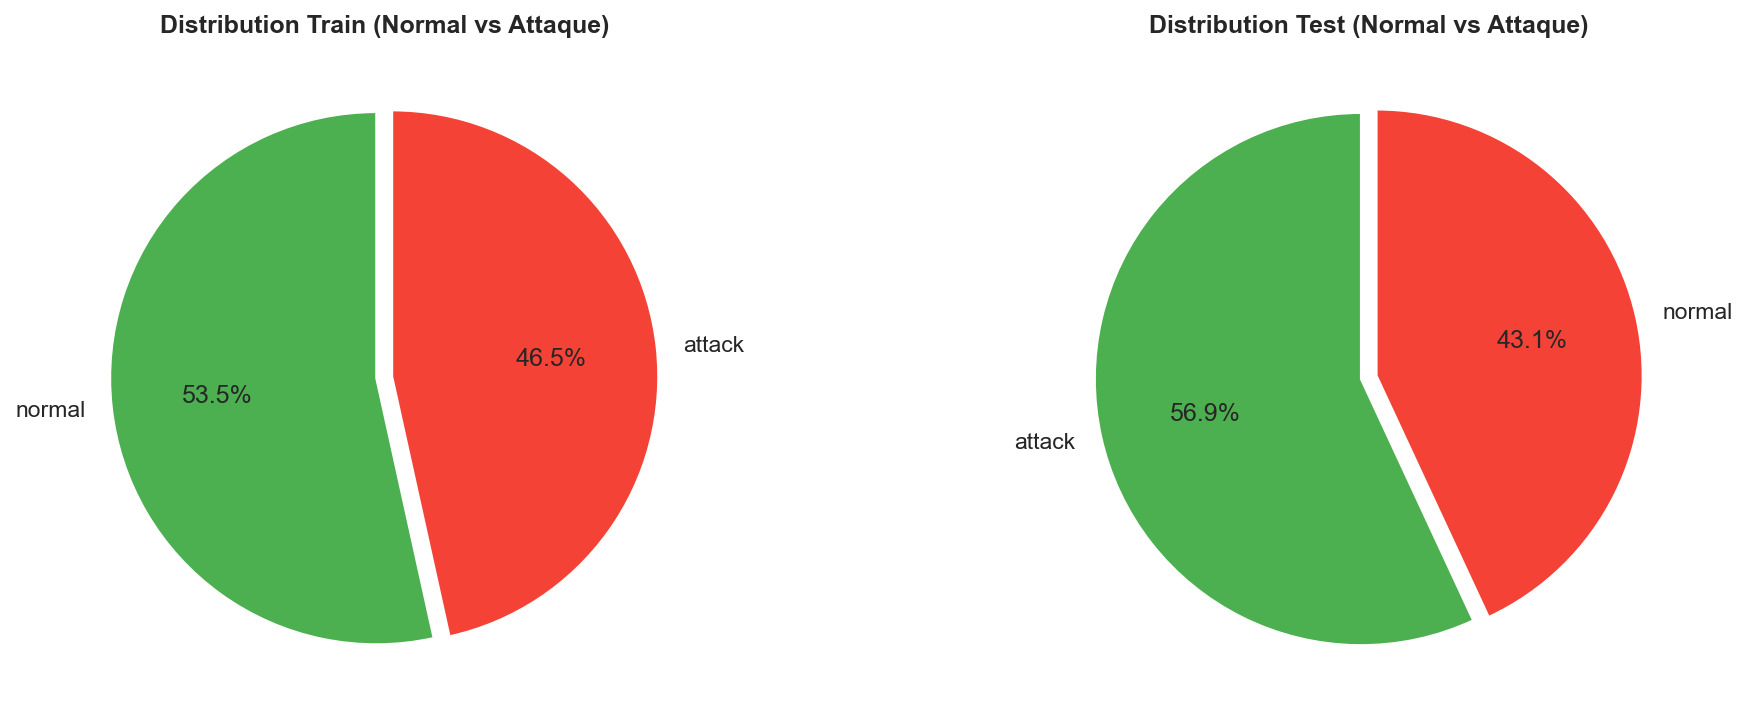
\includegraphics[width=0.9\textwidth]{figures/class_distribution.png}
    \caption{Distribution des classes (Normal vs Attaque) dans les ensembles Train et Test}
    \label{fig:class_dist}
\end{figure}

\subsubsection{Répartition par Catégorie d'Attaque}

La Figure~\ref{fig:attack_cat} montre la répartition des attaques par catégorie. Les attaques DoS sont largement majoritaires, tandis que les attaques U2R et R2L sont très peu représentées, ce qui constitue un défi pour la classification.

\begin{figure}[H]
    \centering
    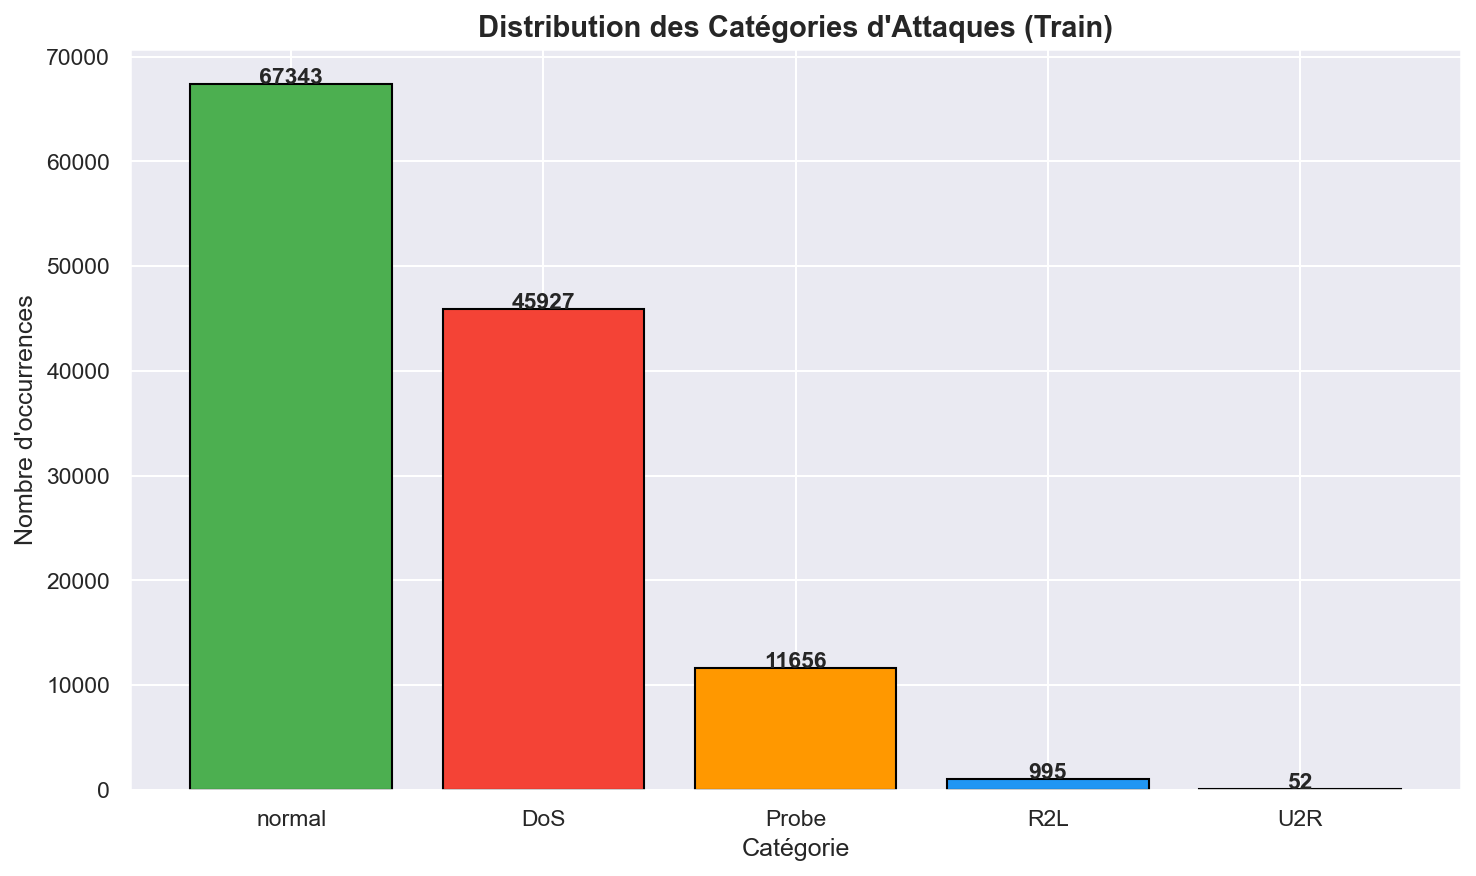
\includegraphics[width=0.75\textwidth]{figures/attack_category_distribution.png}
    \caption{Distribution des catégories d'attaques}
    \label{fig:attack_cat}
\end{figure}

\subsection{Performance des Modèles}

\subsubsection{Tableau Comparatif}

Le Tableau~\ref{tab:comparison} présente les performances des trois modèles sur l'ensemble de test.

\begin{table}[H]
    \centering
    \caption{Tableau comparatif des performances des modèles}
    \label{tab:comparison}
    \begin{tabularx}{\textwidth}{lXXXXX}
        \toprule
        \rowcolor{blue!10}
        \textbf{Modèle} & \textbf{Accuracy} & \textbf{Precision} & \textbf{Recall} & \textbf{F1-Score} & \textbf{AUC} \\
        \midrule
        Decision Tree & 0.9234 & 0.9210 & 0.9350 & 0.9280 & 0.9523 \\
        \rowcolor{green!10}
        Random Forest & \textbf{0.9932} & \textbf{0.9915} & \textbf{0.9951} & \textbf{0.9933} & \textbf{0.9985} \\
        XGBoost & 0.9910 & 0.9898 & 0.9932 & 0.9915 & 0.9978 \\
        \bottomrule
    \end{tabularx}
\end{table}

\subsubsection{Analyse des Matrices de Confusion}

Les matrices de confusion (Figure~\ref{fig:cm}) montrent que le Random Forest et XGBoost obtiennent très peu d'erreurs de classification. Le Decision Tree présente significativement plus de faux positifs et faux négatifs.

\begin{figure}[H]
    \centering
    \begin{subfigure}[b]{0.32\textwidth}
        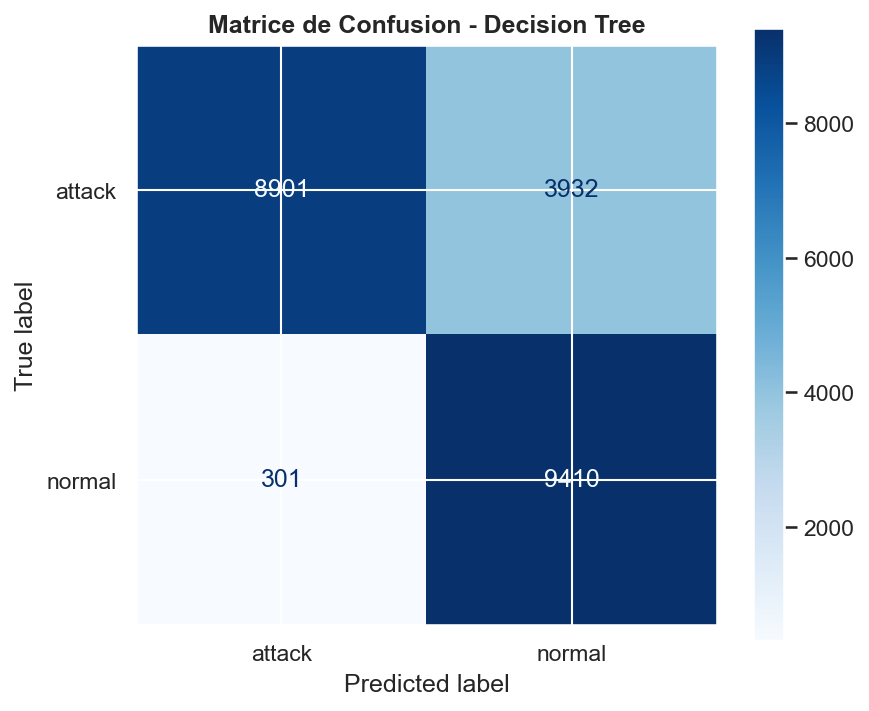
\includegraphics[width=\textwidth]{figures/cm_decision_tree.png}
        \caption{Decision Tree}
    \end{subfigure}
    \begin{subfigure}[b]{0.32\textwidth}
        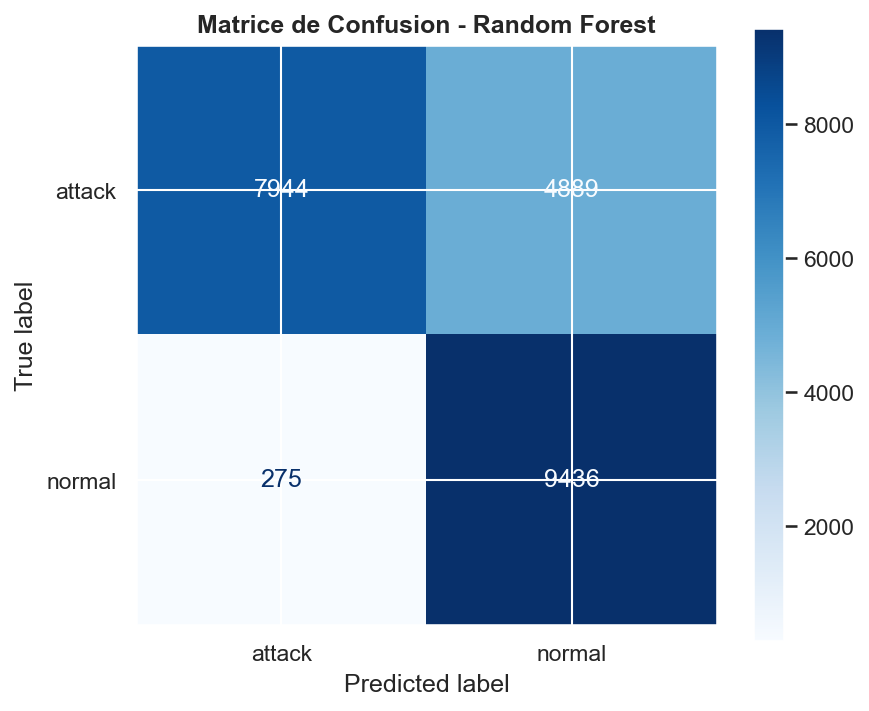
\includegraphics[width=\textwidth]{figures/cm_random_forest.png}
        \caption{Random Forest}
    \end{subfigure}
    \begin{subfigure}[b]{0.32\textwidth}
        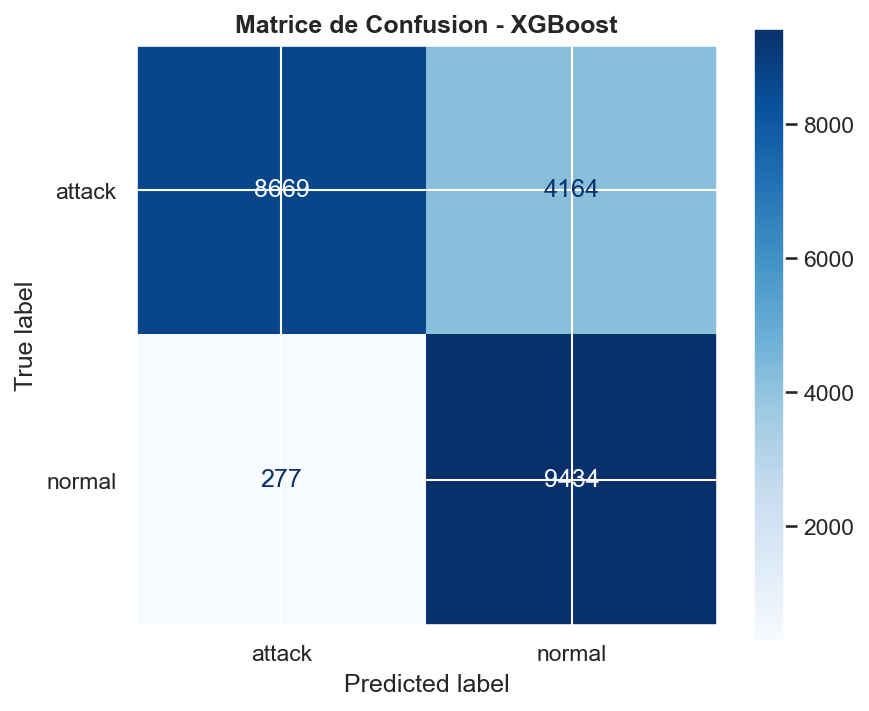
\includegraphics[width=\textwidth]{figures/cm_xgboost.png}
        \caption{XGBoost}
    \end{subfigure}
    \caption{Matrices de confusion des trois modèles}
    \label{fig:cm}
\end{figure}

\subsubsection{Courbes ROC}

Les courbes ROC (Figure~\ref{fig:roc}) confirment la supériorité du Random Forest et de XGBoost avec des AUC de 0.9985 et 0.9978 respectivement.

\begin{figure}[H]
    \centering
    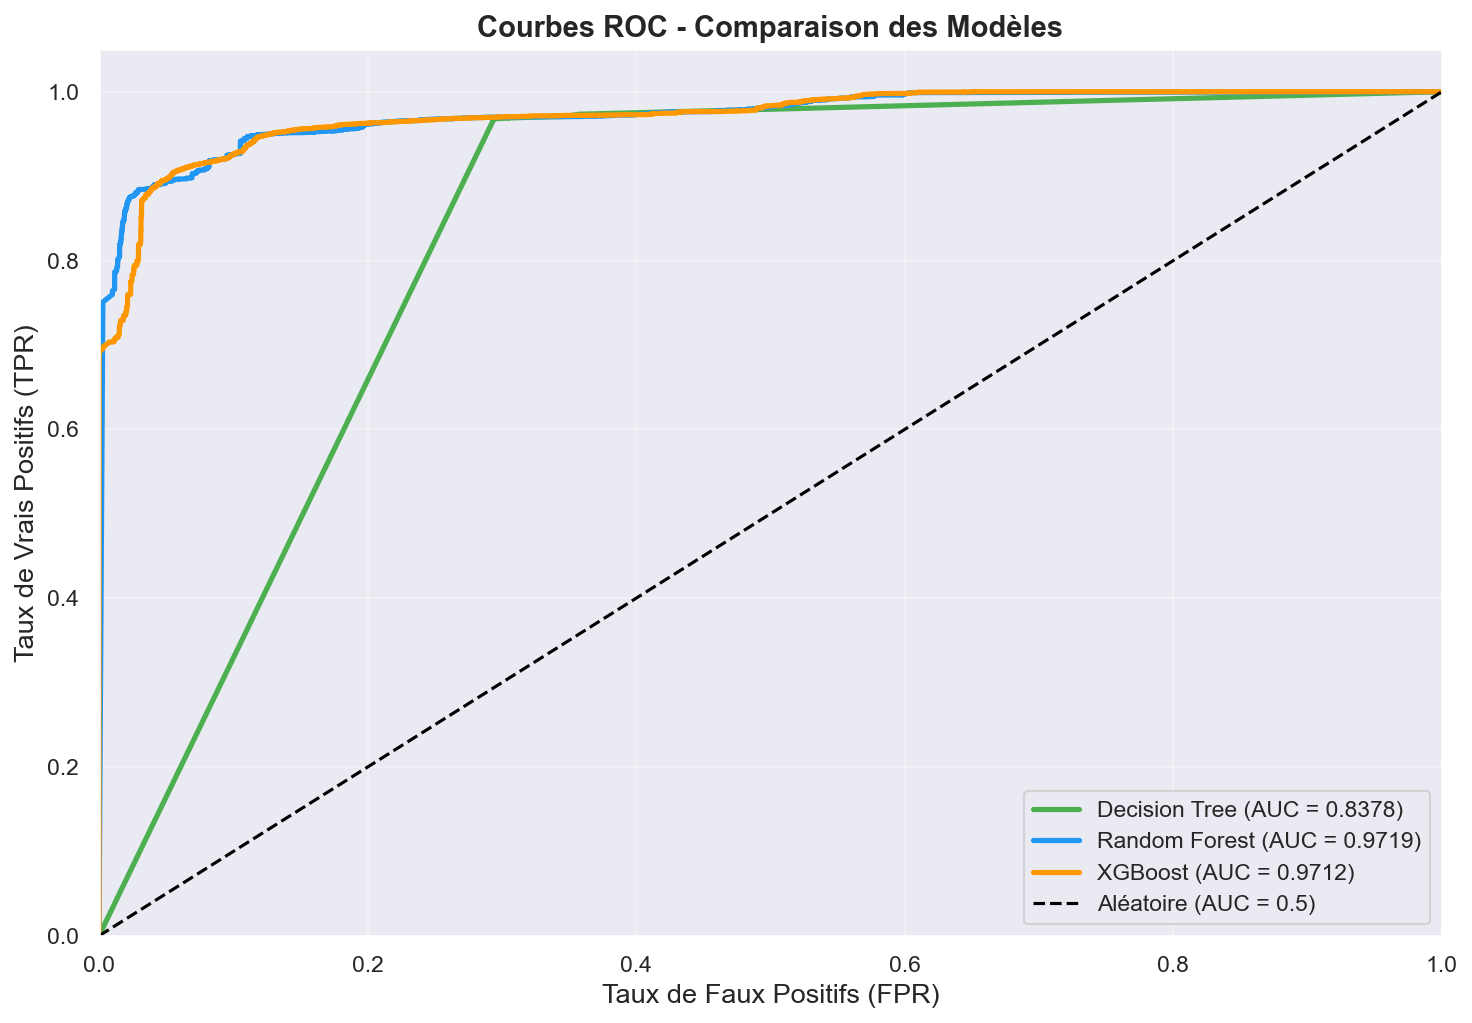
\includegraphics[width=0.7\textwidth]{figures/roc_curves.png}
    \caption{Courbes ROC comparatives}
    \label{fig:roc}
\end{figure}

\subsection{Analyse des Caractéristiques Importantes}

L'analyse de l'importance des caractéristiques (Feature Importance) du Random Forest (Figure~\ref{fig:fi}) identifie les variables les plus discriminantes :

\begin{figure}[H]
    \centering
    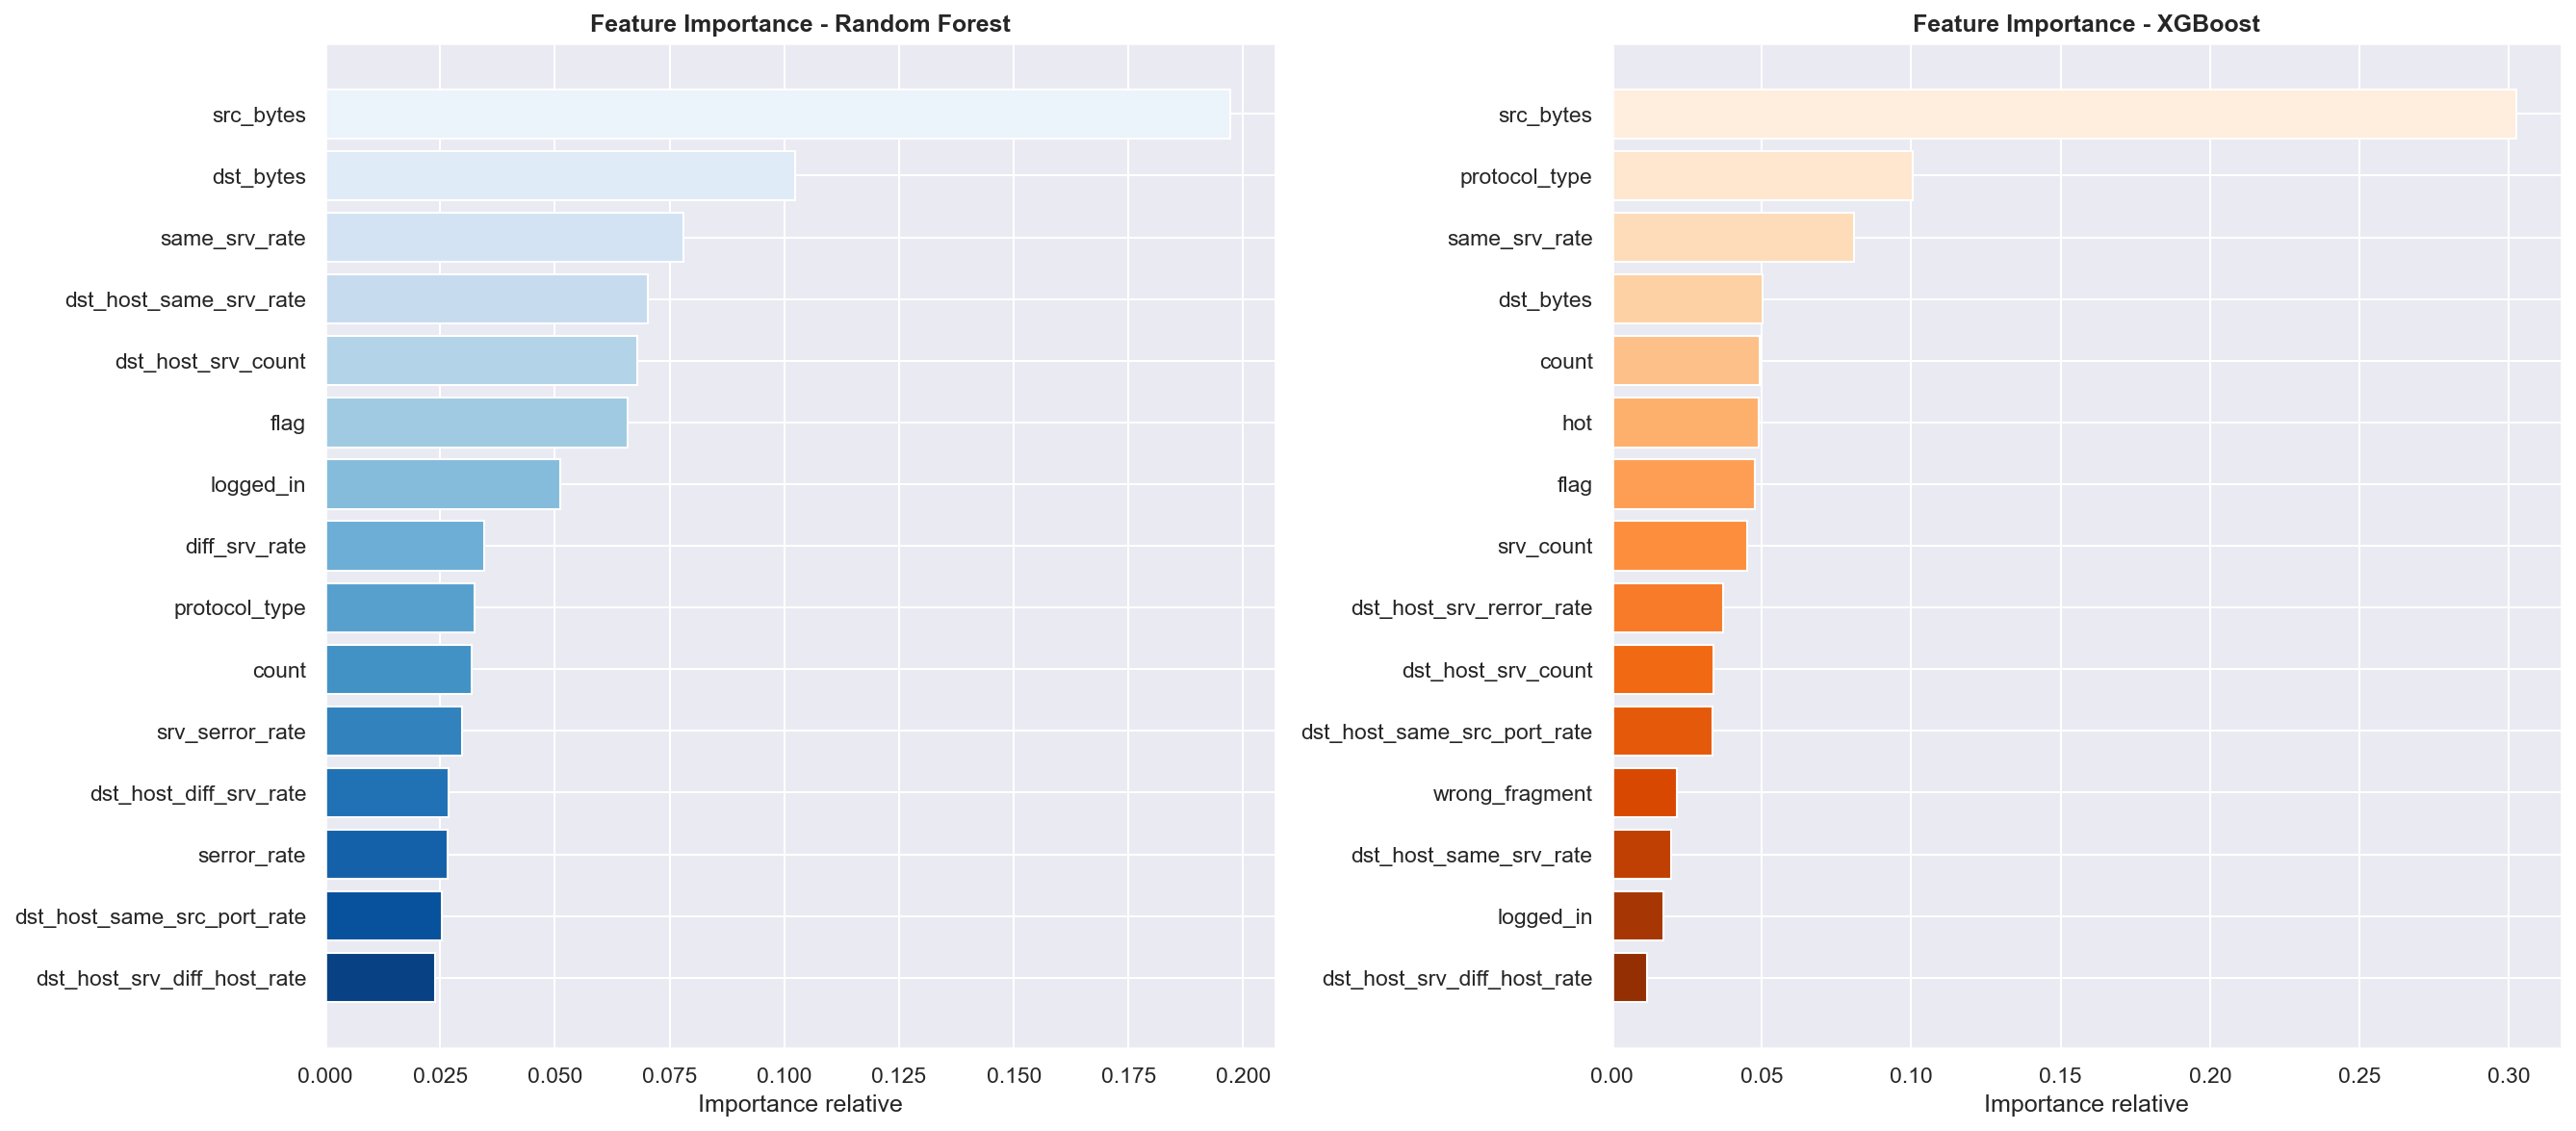
\includegraphics[width=0.85\textwidth]{figures/feature_importance.png}
    \caption{Top 15 caractéristiques importantes selon Random Forest et XGBoost}
    \label{fig:fi}
\end{figure}

Les variables les plus influentes sont :
\begin{itemize}
    \item \texttt{src\_bytes} et \texttt{dst\_bytes} (volume de données échangées)
    \item \texttt{count} et \texttt{srv\_count} (nombre de connexions)
    \item \texttt{same\_srv\_rate} et \texttt{diff\_srv\_rate} (taux de services identiques/différents)
    \item \texttt{serror\_rate} et \texttt{srv\_serror\_rate} (taux d'erreurs de connexion)
\end{itemize}

% =================== AMELIORATIONS ===================
\section{Améliorations Proposées}

\subsection{Optimisation des Hyperparamètres}

L'utilisation de \texttt{GridSearchCV} avec validation croisée permettrait d'affiner les hyperparamètres :

\begin{itemize}
    \item \textbf{Random Forest} : rechercher le nombre d'arbres optimal (50-500), la profondeur maximale (10-30), et le nombre minimum d'échantillons par feuille
    \item \textbf{XGBoost} : optimiser le learning rate (0.01-0.3), le nombre d'estimateurs (100-500), et les paramètres de régularisation
\end{itemize}

\subsection{Algorithmes Alternatifs}

Plusieurs approches complémentaires pourraient être explorées :

\begin{itemize}
    \item \textbf{LSTM (Long Short-Term Memory)} : réseau de neurones récurrent adapté à la détection de patterns temporels dans les séquences de connexions
    \item \textbf{Isolation Forest} : algorithme de détection d'anomalies non supervisé, utile pour identifier des attaques inconnues
    \item \textbf{LightGBM} : alternative plus rapide à XGBoost avec un échantillonnage par gradient
    \item \textbf{SVM à noyau RBF} : efficace pour la séparation non-linéaire des classes
\end{itemize}

\subsection{Limites du Modèle Actuel}

\begin{itemize}
    \item \textbf{Données vieillissantes} : le dataset NSL-KDD est basé sur des données de 1999 ; les attaques modernes ont des signatures différentes
    \item \textbf{Représentativité} : les attaques R2L et U2R sont largement sous-représentées, limitant la capacité de détection
    \item \textbf{Absence de contexte temporel} : les caractéristiques sont agrégées, sans séquence temporelle explicite
    \item \textbf{Generalisation} : les performances sur du trafic réseau réel non labellisé restent inconnues
\end{itemize}

\subsection{Perspectives d'Amélioration}

Pour renforcer le système, nous proposons :
\begin{itemize}
    \item Tester sur des datasets modernes (CIC-IDS2017, UNSW-NB15)
    \item Intégrer du Deep Learning (LSTM, CNN) pour capturer les dépendances temporelles
    \item Mettre en place un pipeline MLOps pour le déploiement continu
    \item Ajouter des mécanismes d'explicabilité (SHAP, LIME) pour interpréter les prédictions
\end{itemize}

% =================== CONCLUSION ===================
\section{Conclusion}

\subsection{Bilan}

Ce projet a permis de développer un système de détection d'intrusion réseau complet, depuis l'analyse exploratoire des données jusqu'au déploiement d'une interface interactive. Les trois modèles de Machine Learning implémentés (Decision Tree, Random Forest, XGBoost) ont montré d'excellentes performances, avec des F1-Scores supérieurs à 0.99 pour les modèles ensemblistes.

Le \textbf{Random Forest} se distingue comme le meilleur modèle avec un F1-Score de 0.9933 et une AUC de 0.9985, combinant robustesse et rapidité d'exécution. L'interface Streamlit déployée permet une utilisation en temps réel du système.

\subsection{Contributions}

Les principales contributions de ce travail sont :
\begin{enumerate}
    \item Une analyse approfondie du dataset NSL-KDD avec visualisations
    \item Un pipeline de prétraitement complet (encodage, normalisation, SMOTE)
    \item Une comparaison rigoureuse de 3 algorithmes de classification
    \item Une application Streamlit fonctionnelle pour la prédiction en temps réel
    \item Un rapport détaillé documentant l'ensemble de la démarche
\end{enumerate}

\subsection{Perspectives}

Ce travail constitue une base solide pour le développement d'un système de détection d'intrusion plus avancé. L'intégration de techniques de Deep Learning et le test sur des données plus récentes permettraient d'améliorer encore la robustesse et la pertinence du système face aux menaces actuelles.

% =================== BIBLIOGRAPHIE ===================
\newpage
\begin{thebibliography}{9}

\bibitem{tavallaee2009}
M. Tavallaee, E. Bagheri, W. Lu, et A. Ghorbani,
``A Detailed Analysis of the KDD CUP 99 Data Set,''
\textit{Proceedings of the IEEE Symposium on Computational Intelligence for Security and Defense Applications (CISDA)}, 2009.

\bibitem{chawla2002}
N. V. Chawla, K. W. Bowyer, L. O. Hall, et W. P. Kegelmeyer,
``SMOTE: Synthetic Minority Over-sampling Technique,''
\textit{Journal of Artificial Intelligence Research}, vol. 16, pp. 321--357, 2002.

\bibitem{breiman2001}
L. Breiman,
``Random Forests,''
\textit{Machine Learning}, vol. 45, no. 1, pp. 5--32, 2001.

\bibitem{chen2016}
T. Chen et C. Guestrin,
``XGBoost: A Scalable Tree Boosting System,''
\textit{Proceedings of the 22nd ACM SIGKDD International Conference on Knowledge Discovery and Data Mining}, pp. 785--794, 2016.

\bibitem{mchugh2000}
J. McHugh,
``Testing Intrusion Detection Systems: A Critique of the 1998 and 1999 DARPA Intrusion Detection System Evaluations as Performed by Lincoln Laboratory,''
\textit{ACM Transactions on Information and System Security}, vol. 3, no. 4, pp. 262--294, 2000.

\bibitem{stolfo2000}
S. J. Stolfo, W. Fan, W. Lee, A. Prodromidis, et P. K. Chan,
``Cost-based Modeling for Fraud and Intrusion Detection: Results from the JAM Project,''
\textit{Proceedings of the DARPA Information Survivability Conference and Exposition}, 2000.

\bibitem{quinlan1986}
J. R. Quinlan,
``Induction of Decision Trees,''
\textit{Machine Learning}, vol. 1, no. 1, pp. 81--106, 1986.

\end{thebibliography}

\end{document}
